\chapter{Experiments and Results}
\label{cha:experimentsandresults}
%---------------------------------------------------------------------------

\section{Song Popularity}
\label{sec:songpopularity}

The analysis of song popularity provides valuable insights into the factors
that influence the success of music tracks. This problem has two approaches:
\begin{itemize}
  \item \textbf{Regression} - Spotify's popularity is a value on scale of
    0-100. This approach involves training a regression model trying to predict
    that value;
  \item \textbf{Classification} - assigning binary label to the songs (popular
    vs. unpopular) and training a classification model to predict it.
\end{itemize}

In this section the prediction of popularity was attempted using several
regression and classification models. These models were trained on different
sets of features, including Spotify metadata, lyrical attributes, and audio
features, with the aim of investigating the predictive power of those features
and their impact on popularity.

Catboost models were used  due to their robustness and performance in handling
complex relationships, as well as ease of use and ability to handle class
imbalance and categorical features out of the box.

Baseline models were also implemented to serve as a reference point:
\begin{itemize}
  \item \textit{Baseline Mean Model}: baseline model for regression that always
    predicts the mean;
  \item \textit{Baseline Majority Model}: baseline model for classification
    that always predicts the majority class;
  \item \textit{Baseline Random Model}: baseline model for classification that
    predicts random class.
\end{itemize}

The experiments involved both quantitative evaluation and SHAP analysis to
assess feature importance and interpretability of the models.

%---------------------------------------------------------------------------
\subsection{Regression Approach}

\begin{center}
\begin{figure}[H]
  \centering
  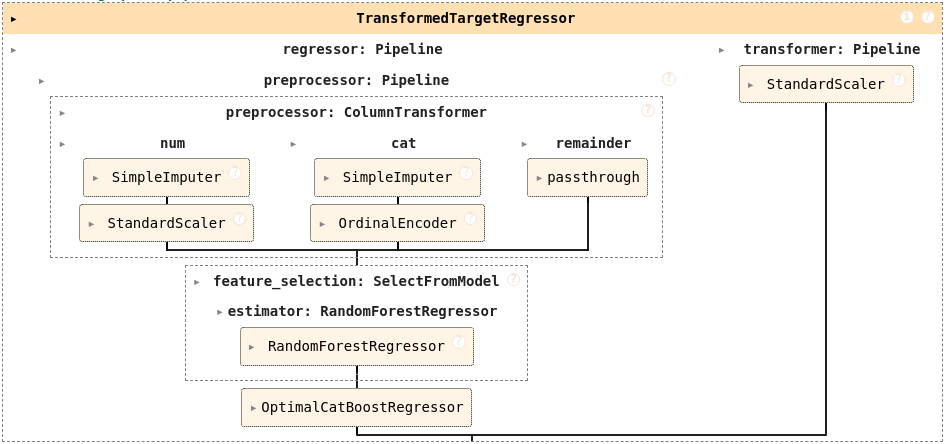
\includegraphics[width=6in]{img/reg_pipeline.png}
  \caption{Regression model pipeline. It involves preprocessing, feature
  selection and CatBoost model.}
  \label{Figure:reg_pipeline}
\end{figure}
\end{center}

The pipeline (fig.~\ref{Figure:reg_pipeline}) was fit with all available features, that
includes Spotify audio features and metadata, lyrical features and features
extracted from the audio files. The feature selection step chose the subset of
most valuable features based on the feature importance from initial Random
Forest model.

\begin{table}[H]
\centering
\caption{Results of regression of popularity.}
\label{Table:regression_popularity}
\begin{tblr}{
  hline{2} = {-}{},
}
 & \textbf{Model}      & \textbf{Features} & \textbf{MAE}  & \textbf{RMSE} & \textbf{$R^2$} \\
 & Baseline Mean Model &                   & 13.53         & 16.90         & -0.01          \\
 & Catboost            & all               & \textbf{6.33} & \textbf{8.52} & \textbf{0.74}  \\
 & Catboost            & lyrical           & 11.81         & 15.29         & 0.17           \\
 & Catboost            & spotify data      & \textbf{6.04} & \textbf{8.10} & \textbf{0.77}  \\
 & Catboost            & audio             & 12.71         & 16.15         & 0.08           
\end{tblr}
\end{table}

As seen in the results table(Tab.~\ref{Table:regression_popularity}), the
CatBoost model trained on Spotify data only achieved the best performance, with
\textbf{Mean Absolute Error (MAE) of \textbf{6.04} and and $R^2$ of 0.77},
closely followed by the model trained on all features that achieved \textbf{MAE
of 6.33 and $R^2$ of 0.74}. The results clearly indicate the importance of
Spotify audio features and metadata in prediction of song's popularity.
Predicting the success  of a musical track based on solely the lyrics or
acoustic features turned out to be diffifcult and models trained on those
subsets of features showed only slight improvement in comparison to the
baseline model. In contrast, the model trained on Spotify data only achieved
\textbf{55.3\%} better MAE score than the baseline model.

Despite feature selection, the model trained on all features performed slightly
worse than the model trained on Spotify features alone. This likely occurred
because adding less important or redundant features reduced the model's ability
to focus on the most relevant Spotify features. Additional noise introduced by
those unnecessary features made it harder to identify clear patterns. This
behavior might also be an indicator of slight overfitting of the model on the
redundant features, even though cross-validation was used to mitigate the risk
of that. Increased regularization could potentially solve this issue in
future experiments.


SHAP analysis was conducted to interpret the predictions of the regression
model and asses the importance of individual features and their contribution to
song's popularity.


\begin{center}
\begin{figure}[H]
  \centering
  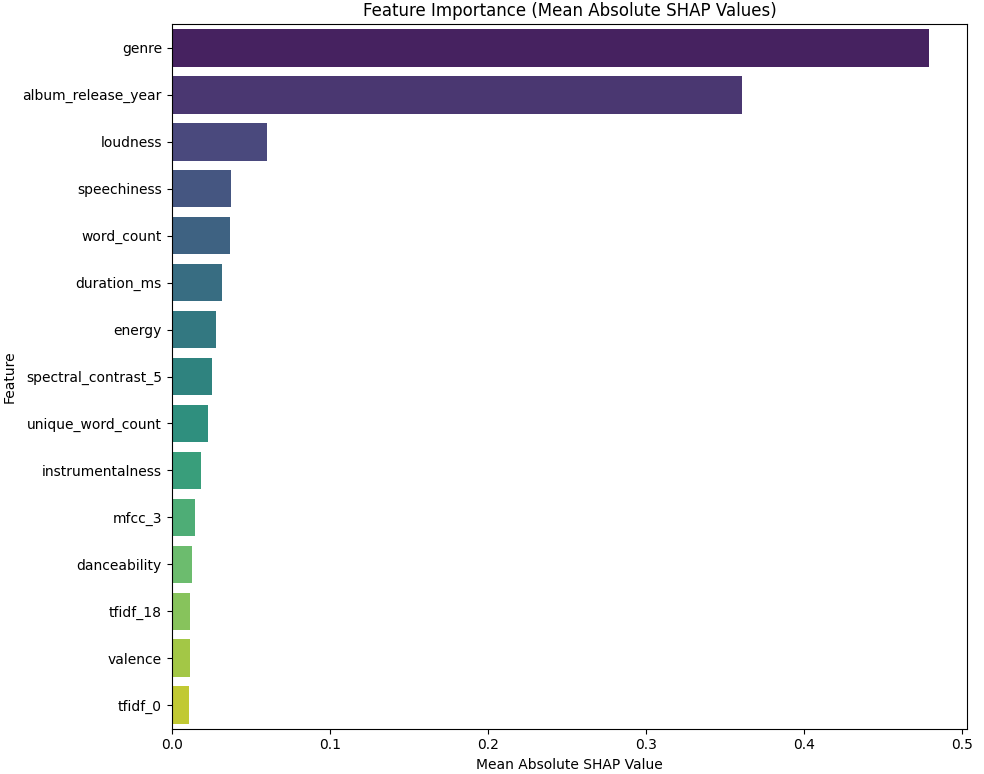
\includegraphics[width=6in]{img/feature_importance_popularity_reg.png}
  \caption{SHAP feature importance plot of the regression model for popularity trained on all features.}
  \label{Figure:feature_importance_popularity_reg}
\end{figure}
\end{center}


The mean absolute SHAP values were used to rank the overall importance of input
features (fig.~\ref{Figure:feature_importance_popularity_reg}). Key insights:
\begin{itemize}
  \item \textbf{Dominance of \textit{Genre} and \textit{Album Release Year}.}:
    these two features account for the majority of the predictive power in the
    model. Genre captures the musical style and release year reflects trends
    and cultural preferences over time;
  \item Spotify's audio features like \textit{loudness} and
    \textit{speechiness} showed moderate contribution to model's performance.
    Their score highlights their relevance in describing popular tracks' audio
    characteristics;
  \item Lyric-based features like \textit{word count} and \textit{unique word
    count} were significantly less impactful, however still contributed to
    model's performance to some degree.
\end{itemize}

\begin{center}
\begin{figure}[H]
  \centering
  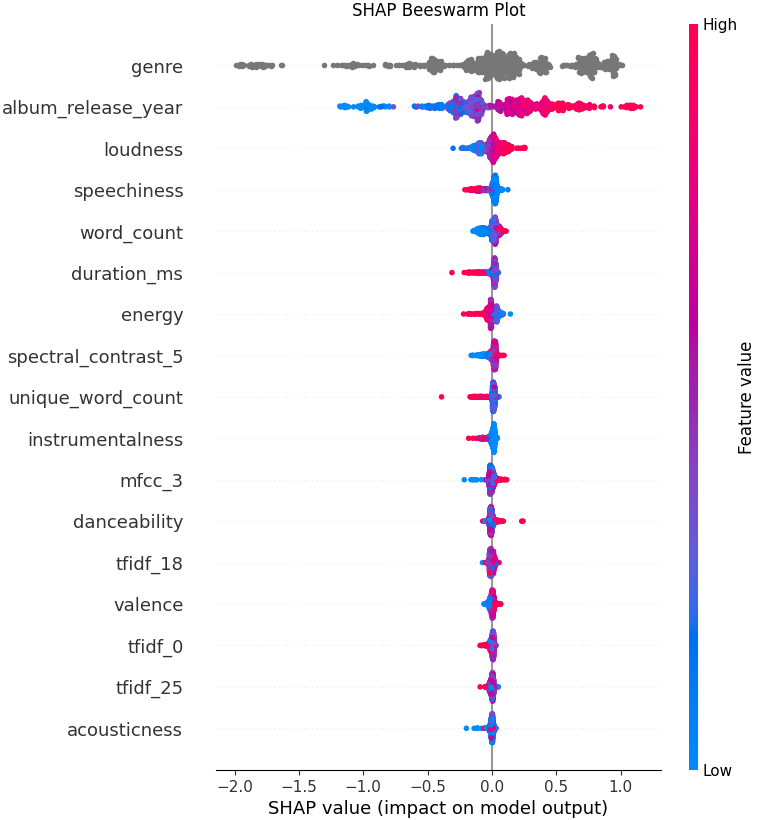
\includegraphics[width=6in]{img/beeswarm_popularity_reg.png}
  \caption{SHAP beeswarm plot of the regression model for popularity trained on all features.}
  \label{Figure:beeswarm_popularity_reg}
\end{figure}
\end{center}

Based on the beeswarm plot (fig.~\ref{Figure:beeswarm_popularity_reg}):
\begin{itemize}
  \item Higher values of \textit{Release Year} correlate with higher values of
    \textit{Popularity}, showing that on average newer songs are more
    popular;
  \item Higher \textit{loudness} and lower \textit{speechiness}
    usually resulted in lower \textit{popularity}.
\end{itemize}



%---------------------------------------------------------------------------
\subsection{Classification Approach}

\begin{center}
\begin{figure}[H]
  \centering
  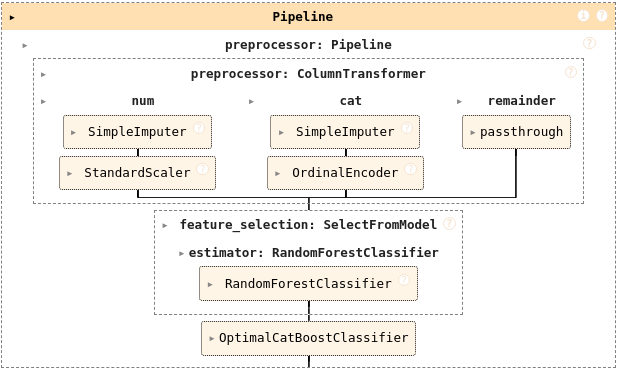
\includegraphics[width=6in]{img/clf_pipeline.png}
  \caption{Classification model pipeline. It involves preprocessing, feature
  selection and CatBoost model.}
  \label{Figure:clf_pipeline}
\end{figure}
\end{center}

The task of predicting song popularity was reformulated as a binary
classification problem (fig.~\ref{Figure:clf_pipeline}) shows the pipeline used
for this task), where the target was to determine whether a song is ``popular''
(1) or ``not popular'' (0). In order to create those labels from an integer
variable with range 0-100, the \textbf{value of 70th percentile of popularity
was used as the threshold}. Songs with popularity higher than the threshold
were labeled as popular and given a value of 1, and the rest was labeled as
unpopular with value 0. This approach based on percentile ensures a balanced
representation of popular songs in the dataset despite the naturally skewed
distribution of popularity scores.

% \usepackage{tabularray}
\begin{table}[H]
\centering
\caption{Results of classification of popularity.}
\label{Table:results_classification_popularity}
\begin{tblr}{
  hline{2} = {-}{},
}
 & \textbf{Model}          & \textbf{Features} & \textbf{Accuracy} & \textbf{F1(w.avg.)} \\
 & Baseline Majority Model &                   & 65.93\%           & 52.39\%             \\
 & Baseline Random Model   &                   & 48.27\%           & 49.57\%             \\
 & Catboost                & all               & \textbf{84.68\%}  & \textbf{84.71\%}    \\
 & Catboost                & lyrical           & 65.79\%           & 64.77\%             \\
 & Catboost                & spotify data      & \textbf{82.06\%}  & \textbf{82.32\%}    \\
 & Catboost                & audio             & 63.17\%           & 63.00\%             
\end{tblr}
\end{table}


The models, as shown in the table
Tab.~\ref{Table:results_classification_popularity} were evaluated based on
accuracy and weighted F1-score. \textit{Baseline Majority Model} (it predicts
the majority class for all samples) achieved an accuracy of 65.93\% and an
F1-score of 52.39\%. Lower value of F1-score shows that it wasn't able to
correctly handle the class imbalance introduced by the thresholding.

The \textit{Baseline Random Model} (guesses classes randomly), performed worse
than the previous one, with accuracy of 48.27\% and F1-score of 49.57\%.

CatBoost model significantly outperformed both baselines, achieving an overall
accuracy of 84.68\% and a weighted F1-score of 84.71\% when trained on all
features. Its superior performance shows the strong predictive power of all the
features combined and the ability to handle imbalanced data.

The CatBoost model trained on Spotify data performed quite well, with an accuracy of
82.06\% and an F1-score of 82.32\%, showing that Spotify features alone provide
strong predictive power. Nevertheless, the model trained on all features
managed to slightly outperform it, suggesting that additional features apart from
the Spotify data  provide some complementary information.

The model using only lyrical features achieved an accuracy of 65.79\%, which is
slightly lower than the \textit{Baseline Majority Model}, but a higher F1-score
of 64.77\%, reflecting its ability to handle class imbalance better than the
majority model. This confirms that lyrical features are limited in their
ability to predict song popularity.


The performance of the model trained on features extracted from audio files was
similarly bad as of the lyrical one, showing that audio features alone are 
poor predictors of song's popularity.


SHAP analysis revealed that \textit{genre}, \textit{album release year} and
\textit{loudness} were the most significant predictors of
popularity (fig.~\ref{Figure:feature_importance_popularity_clf}). The results are
similar to the ones obtained in the regression approach, highlighting the
utility of  these features across different modelling approaches. This finding
confirms their central role in understanding and predicting song success.

\begin{center}
\begin{figure}[H]
  \centering
  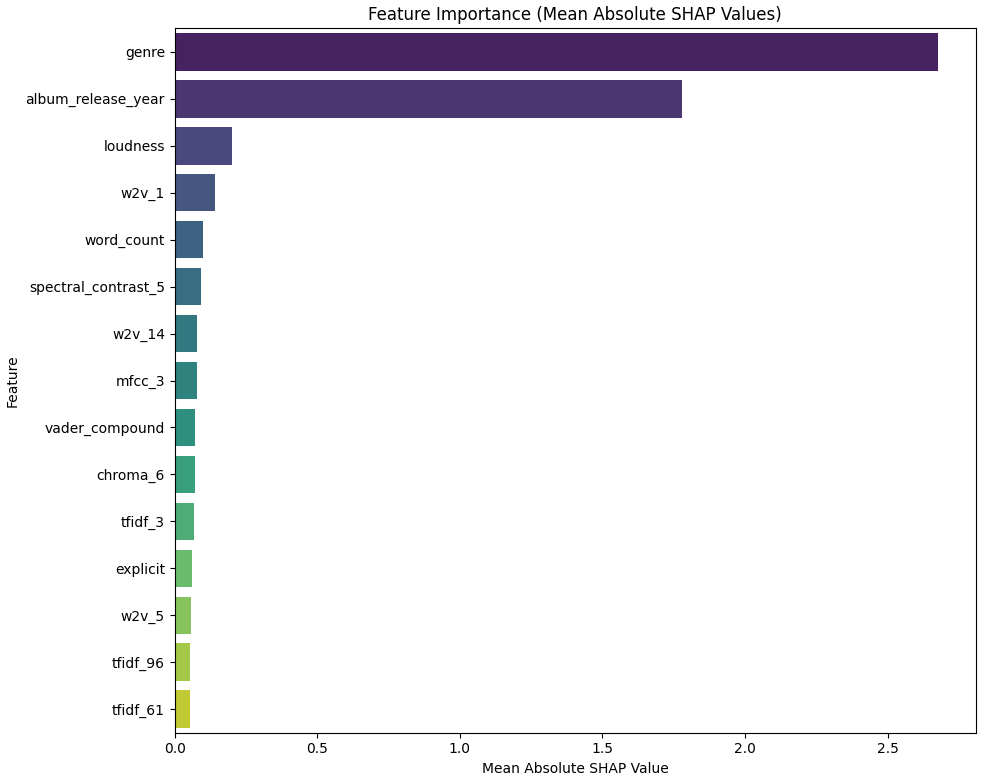
\includegraphics[width=6in]{img/feature_importance_popularity_clf.png}
  \caption{SHAP feature importance plot of the classification model for popularity trained on all features.}
  \label{Figure:feature_importance_popularity_clf}
\end{figure}
\end{center}

\begin{center}
\begin{figure}[H]
  \centering
  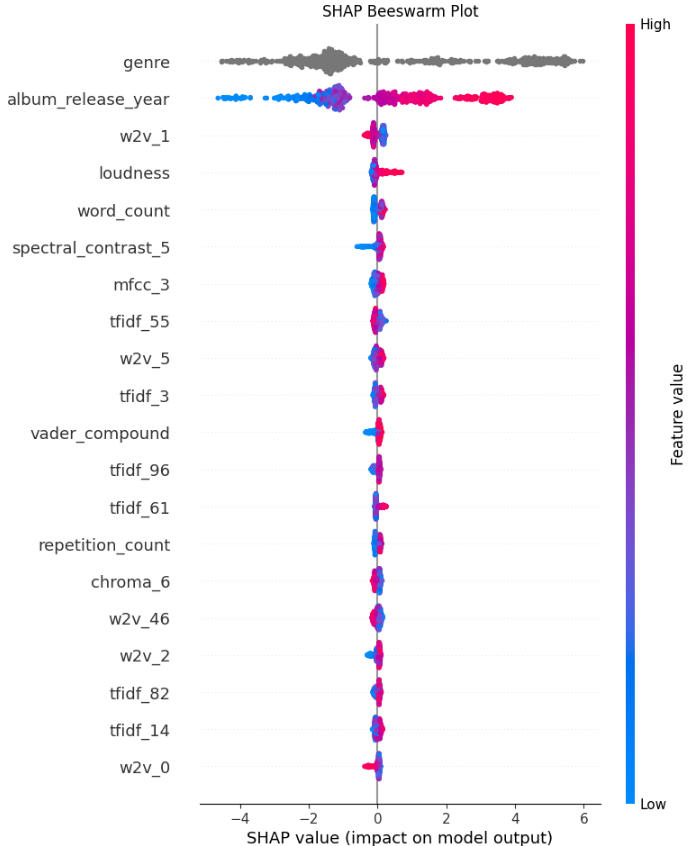
\includegraphics[width=6in]{img/beeswarm_popularity_clf.png}
  \caption{SHAP beeswarm plot of the classification model for popularity trained on all features.}
  \label{Figure:beeswarm_popularity_clf}
\end{figure}
\end{center}


Based on the feature
importance (fig.~\ref{Figure:feature_importance_popularity_reg} and
fig.~\ref{Figure:feature_importance_popularity_clf}) and beeswarm
plots (fig.~\ref{Figure:beeswarm_popularity_reg} and
fig.~\ref{Figure:beeswarm_popularity_clf}) produced by SHAP, several differences
between regression and classification model can be observed:
\begin{itemize}
  \item Lyrics embeddings (TF-IDF and Word2Vec) played a slightly bigger role in
    the classification model;
  \item Classification model seemed to pay much less attention to Spotify audio
    features, like \textit{danceability}, \textit{energy} and
    \textit{speechiness} in comparison to the regression one;
  \item Unlike in regression, in classification a sentiment metric,
    \textit{VADER compound} contributed to the prediction of popularity. More
    popular songs tend to have more positive lyrics.
\end{itemize}


%---------------------------------------------------------------------------
\section{Explicitness}
\label{sec:explicitness}

\subsection{Classification Approach}
The task of predicting whether a song contains explicit content was approached
as a classification problem. The performance of the CatBoost model was compared
against baseline on different feature subsets. One of the key challenges of
this problem was significant class imbalance present in the dataset;
approximately 85\% of the songs did not contain explicit content.

Significant class imbalance can lead to models favoring the majority class,
potentially resulting in  high accuracy but poor performance on the minority
class. To address this problem, CatBoost's class weights parameter was used.
This parameter allowed the model to penalize misclassifications of the minority
class more heavily, therefore improving its ability to recognize explicit
content.

% \usepackage{tabularray}
\begin{table}[H]
\centering
\caption{Results of classification of explicitness.}
\label{Table:results_classification_explicitness}
\begin{tblr}{
  hline{2} = {-}{},
}
 & \textbf{Model}          & \textbf{Features} & \textbf{Accuracy} & \textbf{F1 weighted average} \\
 & Baseline Majority Model &                   & 84.00\%           & 76.69\%                      \\
 & Baseline Random Model   &                   & 47.03\%           & 53.91\%                      \\
 & Catboost                & all               & \textbf{92.41\%}  & \textbf{92.40\%}             \\
 & Catboost                & lyrical           & \textbf{92.41\%}  & \textbf{92.25\%}             \\
 & Catboost                & spotify data      & 86.48\%           & 87.11\%                      \\
 & Catboost                & audio             & 82.75\%           & 82.47\%                      
\end{tblr}
\end{table}


The table(Tab.~\ref{Table:results_classification_explicitness}) presents the
results of the models evaluation with accuracy and weighted F1 score. The
Baseline Majority Model achieved accuracy of 84\% and significantly lower F1
weighted average of 76.69\%, which is due to the imbalance in the data. The
\textit{Baseline Random Model} performed very poorly, with an accuracy of
47.03\% and F1 weighted average of 53.91\%.

In contrast, the CatBoost model outperformed both baselines achieving accuracy
of \textbf{92.41\%} and weighted average score of \textbf{92.4\%} when trained
on all features. The model trained on lyrical features only performed nearly as
well, hinting that explicitness can largely be predicted based on lyrical
content. 

Models that relied on Spotify metadata and features extracted from
audio files achieved lower performance, with accuracy close to \textit{Baseline
Majority Model}, but with higher F1 scores, due to their ability to address
class imbalance. These observations show that the features that these models
were trained on are not sufficient to predict presence of explicit content
in songs.


\begin{center}
\begin{figure}[H]
  \centering
  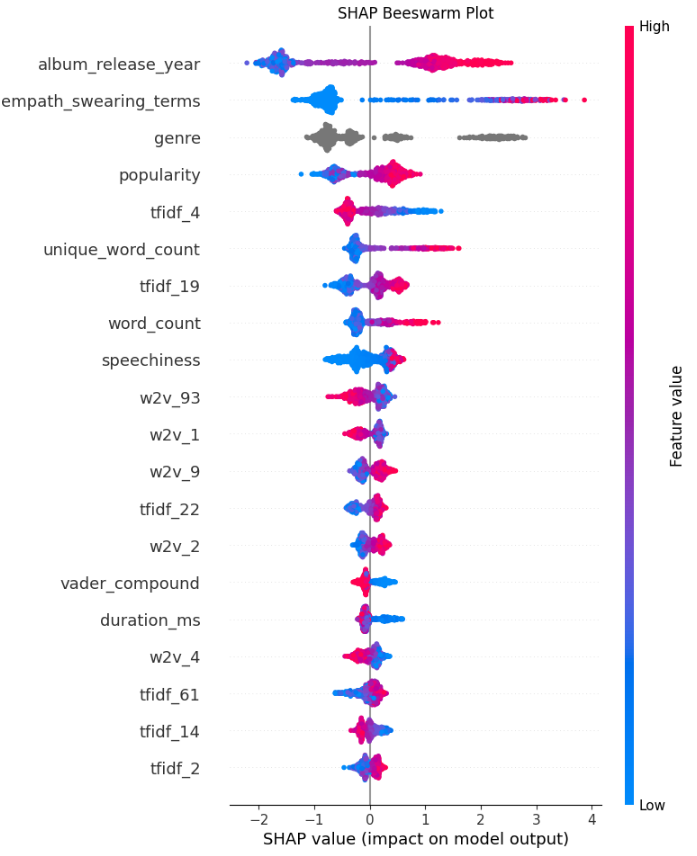
\includegraphics[width=6in]{img/beeswarm_explicitness.png}
  \caption{SHAP beeswarm plot of the classification model for explicitness
  trained on all features.}
  \label{Figure:beeswarm_explicitness}
\end{figure}
\end{center}

\begin{center}
\begin{figure}[H]
  \centering
  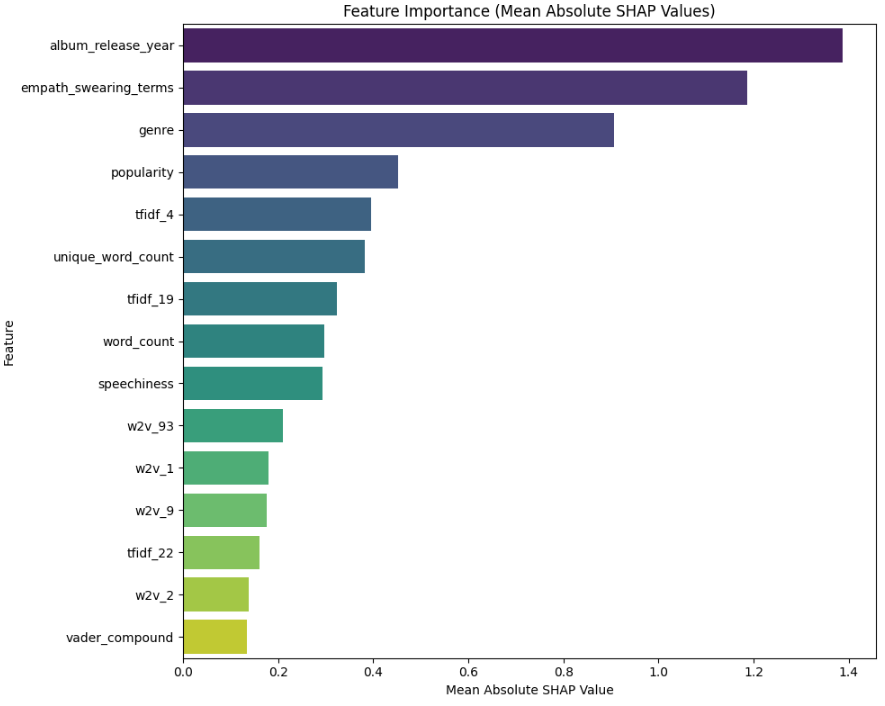
\includegraphics[width=6in]{img/feature_importance_explicitness.png}
  \caption{SHAP feature importance plot of the classification model for
  explicitness  trained on all features.}
  \label{Figure:feature_importance_explicitness}
\end{figure}
\end{center}


Based on the SHAP analysis (fig.~\ref{Figure:beeswarm_explicitness},
fig.~\ref{Figure:feature_importance_explicitness}) we can observe that the key
features for this task turned out to be:
\begin{itemize}
  \item \textbf{Album Release Year}: this feature had  highest feature
    importance, reflecting temporal trends in explicit content. Newer songs are
    statistically more likely to contain explicit language, reflecting changing
    societal norms and artistic expressions over time;
  \item \textbf{Empath Swearing Terms}: As expected, the presence of swearing
    terms was a strong indicator of explicitness;
  \item \textbf{Genre} was the third most important feature, showing that
    certain genres  are more likely to contain explicit content than others;
  \item \textbf{TF-IDF}: several vectors created using TF-IDF and later reduced
    via PCA significantly contributed to the model's predictions. Similar to
    the Empath feature, TF-IDF likely captured swear words and related patterns
    in the lyrics, reinforcing its importance;
  \item \textbf{Speechiness}: songs with higher values of
    speechiness—indicating a greater presence of spoken-word elements—were more
    likely to be labeled as explicit.
\end{itemize}




The task of predicting explicitness could potentially achieve higher
performance by leveraging the interpretability of explicitness, which provides
clear hints about the most relevant features for this property. However, the
primary goal of this analysis was not to maximize model performance but to
explore the impact of various feature subsets on the prediction of
explicitness.

The results indicate that predicting explicitness based solely on audio
features is inherently challenging. The model trained on audio features
performed worse than the baseline, suggesting that the extracted audio
characteristics from the MP3 files do not sufficiently capture the explicit
nature of songs. This highlights the need for features more directly related to
lyrical or contextual information when modeling explicit content.



%---------------------------------------------------------------------------
\subsection{Impact of Explicit Language on Popularity and Sentiment}
\label{sec:explicitmorepopular}

To investigate the relationship between explicitness and song's popularity, a
bootstrap test was conducted. Bootstrap was chosen for this purpose due to its
flexibility, because unlike other, traditional parametric tests, bootstrap does
not rely on strong assumptions about the underlying data distribution. That's
why its well-suited for analyses on real-world datasets, that may not meet
strict requirements.



\begin{center}
\begin{figure}[H]
  \centering
  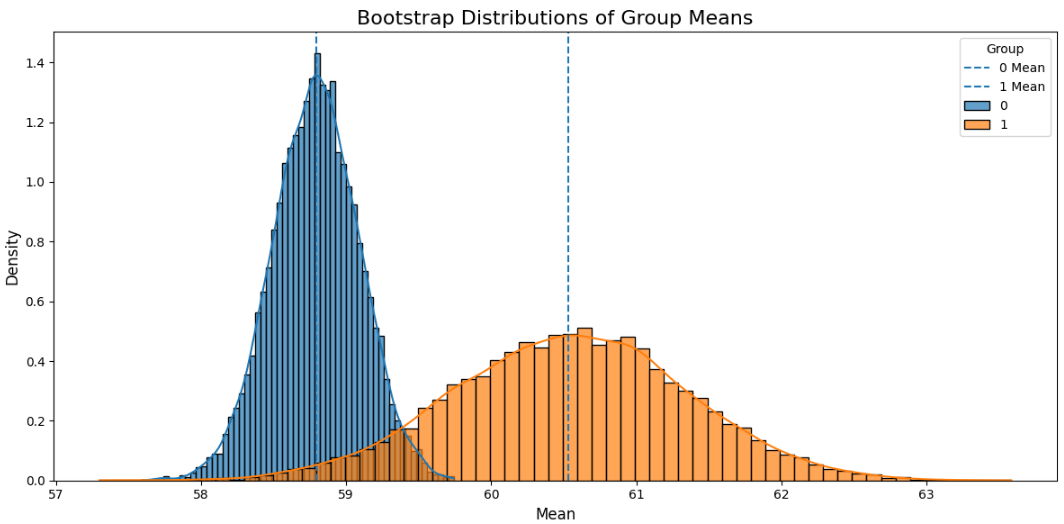
\includegraphics[width=6in]{img/explicitness_bootstrap.png}
  \caption{Bootstrap Test to check if explicit songs are on average more
  popular.}
  \label{Figure:explicitness_bootstrap}
\end{figure}
\end{center}



\begin{center}
\begin{figure}[H]
  \centering
  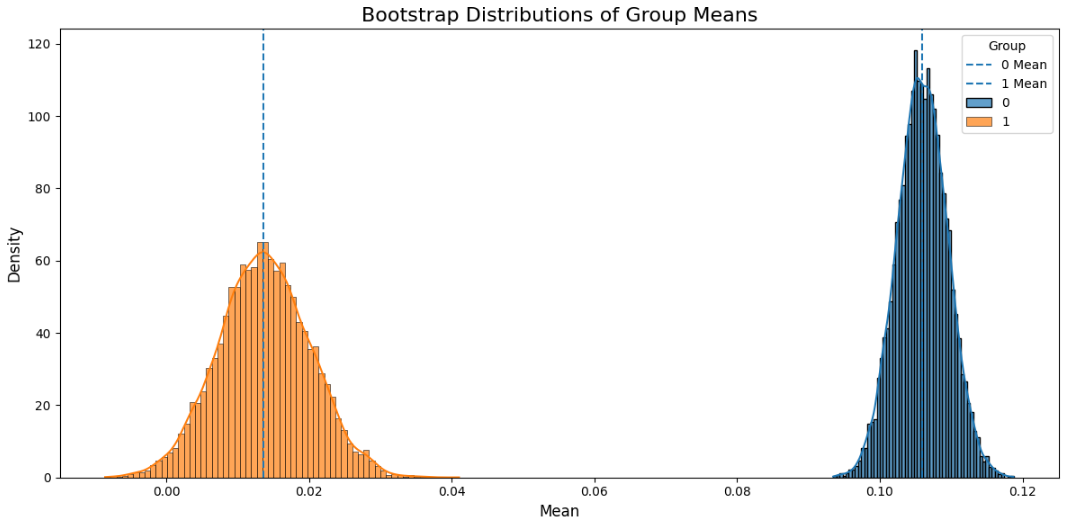
\includegraphics[width=6in]{img/explicitness_bootstrap_2.png}
  \caption{Bootstrap Test to check if explicit songs are on average more
  positive or negative than non-explicit songs.}
  \label{Figure:explicitness_bootstrap_2}
\end{figure}
\end{center}



\begin{table}[H]
\centering
\caption{Results of the Bootstrap Test.}
\label{Table:bootstrap_results}
\resizebox{\linewidth}{!}    & 0.08\%                  & 5.79\%                           & 1.74               & 0.0453                        & 3.4013                        \\
Sentiment~ Polarity & non-explicit           & explicit                 & \textbf{-87.10\%}  & -100.69\%               & -73.63\%                         & -0.09              & -0.1067                       & -0.0780                       
\end{tblr}
}
\end{table}

The analysis results (Tab.~\ref{Table:bootstrap_results},
fig.~\ref{Figure:explicitness_bootstrap}) reveal that explicit songs are, on
average, \textbf{2.96\%} more popular than non-explicit songs. The confidence
interval of [0.08\%, 5.79\%] suggests statistically significant but modest
increase in popularity for explicit songs.

For sentiment polarity, the results (Tab.~\ref{Table:bootstrap_results},
fig.~\ref{Figure:explicitness_bootstrap_2}) show that explicit songs are on average
\textbf{87.10\%} less positive than non-explicit songs. The confidence interval
of [-100.69\%, 73.63\%] confirms it to be a very significant difference.
Explicit songs may reflect more intense, provocative or aggresive themes, which
may carry less positive emotion.


%---------------------------------------------------------------------------
\section{Sentiment}
\label{sec:sentiment}
\begin{center}
\begin{figure}[H]
  \centering
  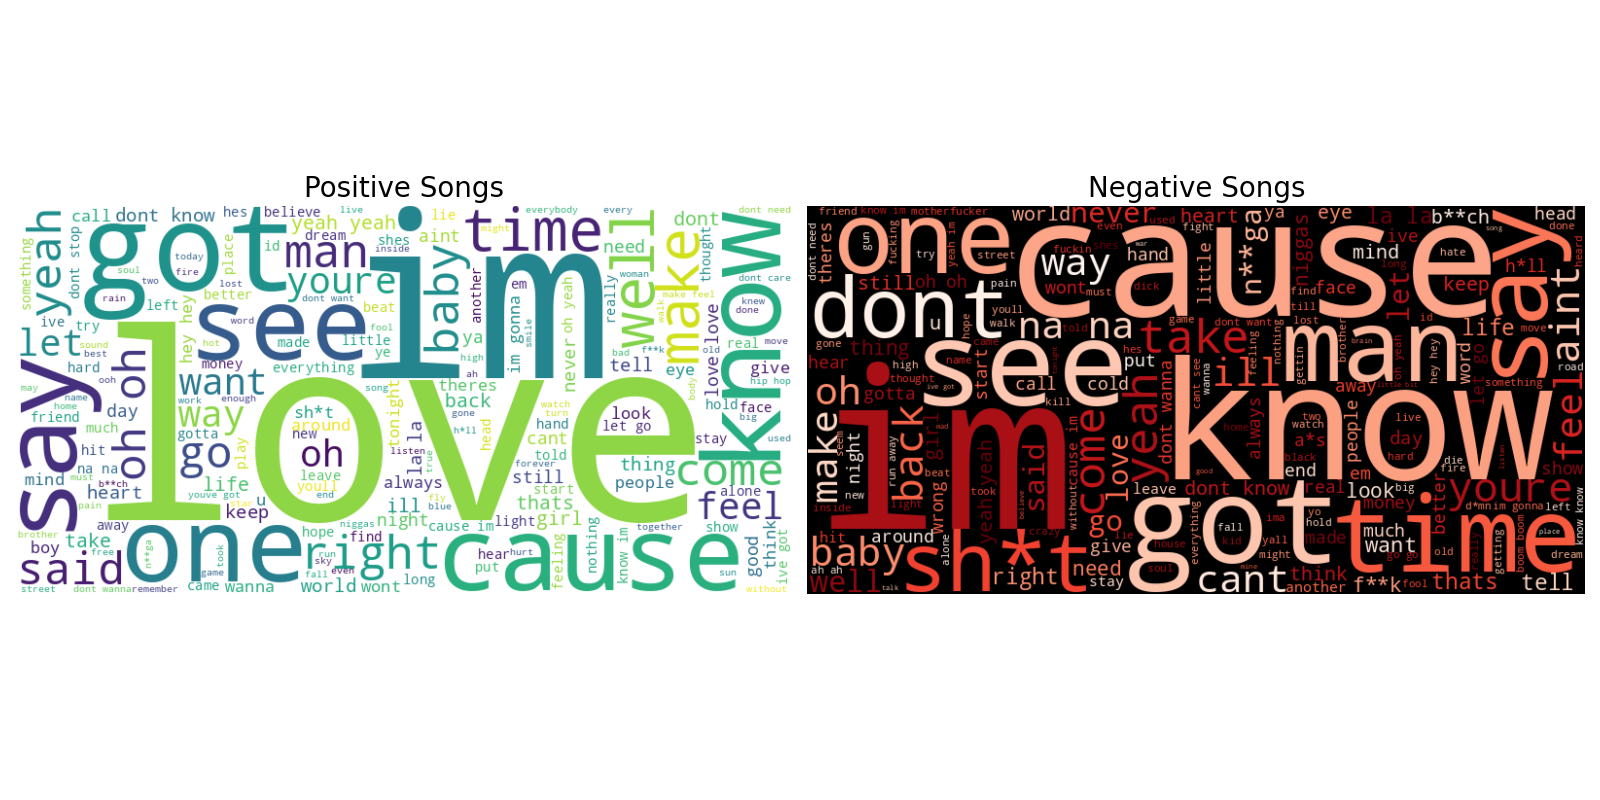
\includegraphics[width=7in]{img/wordclouds.png}
  \caption{Wordclouds of Positive and Negative Sentiment Songs.}
  \label{Figure:wordclouds}
\end{figure}
\end{center}

This section tackles the problem of song lyrics sentiment prediction. The
binary sentiment labels (positive (1) and negative (0)) were derived from the
variable \textit{sentiment polarity}. Songs with polarity values below 0 were
labeled as negative, while those above 0 were labeled as positive. The wordclouds
on figure fig.~\ref{Figure:wordclouds} show most promiment words for 
songs labeled as positive and negative.


This process resulted in an unbalanced target variable, where the positive
class was overrepresented. Additionally, due to the left-skewed distribution of
\textit{sentiment polarity}, songs labeled as \textit{positive} were, on
average, more strongly positive compared to the relatively moderate
\textit{negativity} of songs in the negative class. 

While this bias in class definition might pose challenges for traditional
predictive modeling, it's not a major concern for this study. The primary
objective of this experiment is to understand which factors contribute to
song’s positivity, not achieving perfect predictive accuracy. Chosen approach
provides sufficient insight into the relationship between song features and
sentiment.


\begin{table}[H]
\centering
\caption{Results of classification of sentiment.}
\label{Table:results_sentiment}
\begin{tblr}{
  hline{2} = {-}{},
}
 & \textbf{Model}          & \textbf{Features} & \textbf{Accuracy} & \textbf{F1(w.avg.)} \\
 & Baseline Majority Model &                   & 69.65\%           & 57.19\%             \\
 & Baseline Random Model   &                   & 52.55\%           & 54.46\%             \\
 & Catboost                & all               & 71.44\%           & 69.77\%             \\
 & Catboost                & lyrical           & \textbf{71.86\%}  & \textbf{70.72\%}    \\
 & Catboost                & spotify data      & 67.44\%           & 64.94\%             \\
 & Catboost                & audio             & 65.10\%           & 63.43\%             
\end{tblr}
\end{table}


The results(Tab.~\ref{Table:results_sentiment}) show that the Catboost models
outperformed the baselines significantly. Among  them, the one trained only on
lyrical features performed the best, with accuracy of 71.86\% and weighted
F1-score of 70.72\%. The result shows the importance of lyrical features in
sentiment prediction. The dominance of lyrical features might be caused by the
fact that the target variable was derived from lyrics, and songs with positive
lyrics don't necessarily have to be positive overall.

The model trained on all features followed the one trained on lyrical features
closely, but performed slightly worse due to large amount of redundant
features, despite the presence of feature selection step in the pipeline that
attempted to discard them. Models trained on only Spotify or audio features
performed worse, achieving accuracies of 67.44\% and 65.10\%, respectively.

These results suggest that Spotify features and the features extracted from MP3
files are to some extent indicative of the sentiment, but much less in
comparison to the lyrical data. Future work could focus on advanced feature
engineering or exploring additional audio-based properties to improve the
performance of audio-based sentiment prediction models.


\begin{center}
\begin{figure}[H]
  \centering
  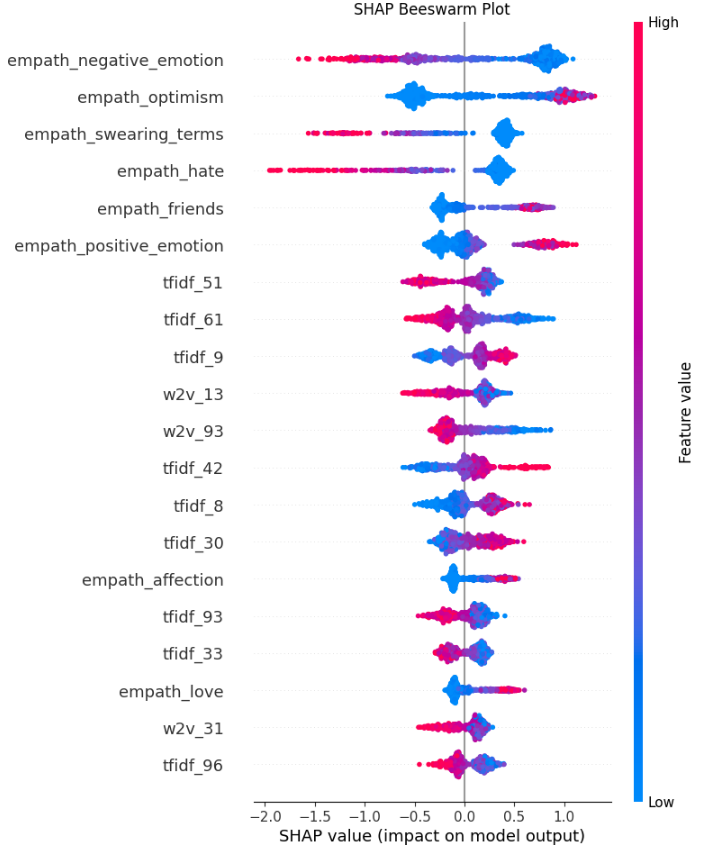
\includegraphics[width=6in]{img/beeswarm_sentiment.png}
  \caption{SHAP beeswarm plot of the classification model for sentiment
  trained on all features.}
  \label{Figure:beeswarm_sentiment}
\end{figure}
\end{center}

\begin{center}
\begin{figure}[H]
  \centering
  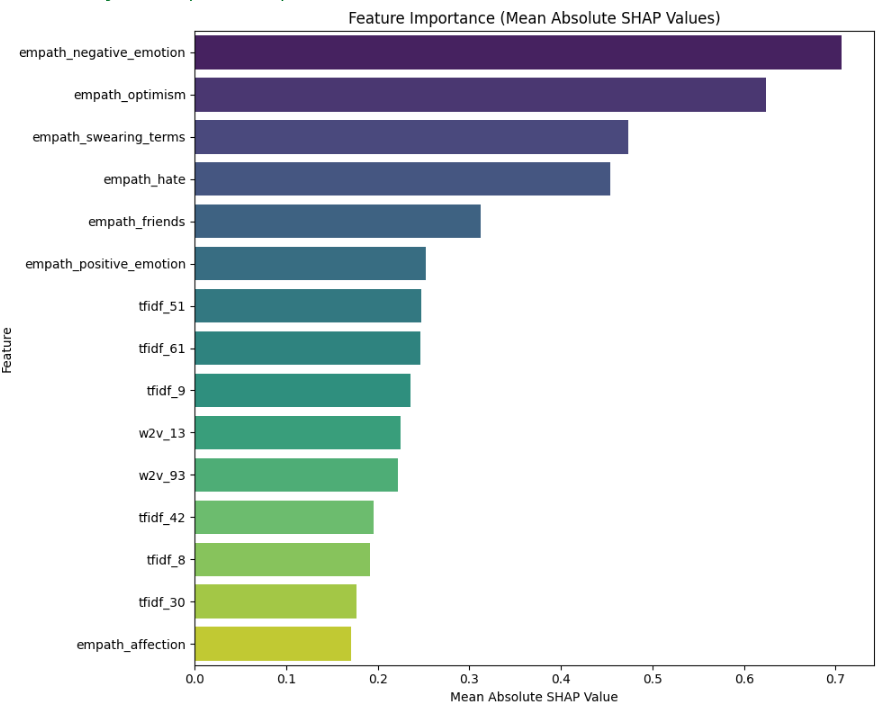
\includegraphics[width=6in]{img/feature_importance_sentiment.png}
  \caption{SHAP feature importance plot of the classification model for
  sentiment trained on all features.}
  \label{Figure:feature_importance_sentiment}
\end{figure}
\end{center}

The SHAP analysis showed that lyrical features,
like were the most influential in predicting sentiment, with negative emotions
and swearing linked to negative sentiment, and optimism and positive emotion
tied to positive sentiment. TF-IDF and Word2Vec embeddings also contributed,
reflecting patterns in lyrics. Audio features, however, had minimal impact,
emphasizing the need for improved audio feature engineering to capture
sentiment.

The feature importance (fig.~\ref{Figure:feature_importance_sentiment}) and
beeswarm (fig.~\ref{Figure:beeswarm_sentiment}) plots show that empath
features, like \textit{empath negative emotion}, \textit{empath optimism}, and
\textit{empath swearing terms}, were the most important in prediction of
sentiment. TF-IDF and Word2Vec embeddings also contributed significantly,
reflecting patterns in lyrics. Audio features had minimal impact, emphasizing
the need to extend audio feature engineering to find features that better
capture sentiment.

%---------------------------------------------------------------------------
\section{Genre}
\label{sec:genre}

The objective of this experiment is classification of song's genre on different
feature subsets. The dataset includes 10 genres, covering a diverse range of
musical styles.

\begin{table}[H]
\centering
\caption{Results of classification of genre.}
\label{Table:results_genre}
\resizebox{\linewidth}{!}{%
\begin{tblr}{
  hline{2} = {-}{},
}
 & \textbf{Model}          & \textbf{Features} & \textbf{Accuracy} & \textbf{F1(w.avg.)} \\
 & Baseline Majority Model &                   & 11.17\%           & 02.24\%             \\
 & Baseline Random Model   &                   & 10.20\%           & 10.38\%             \\
 & Catboost                & all               & \textbf{61.24\%}  & \textbf{60.27\%}    \\
 & Catboost                & lyrical           & 32.96\%           & 32.23\%             \\
 & Catboost                & spotify data      & 56.96\%           & 56.65\%             \\
 & Catboost                & audio             & 31.31\%           & 30.33\%             
\end{tblr}
}
\end{table}

The results of the experiment are presented in table
Tab.~\ref{Table:results_genre}. The baseline models achieved very poor
performance. The \textit{Baseline Majority Model} achieved accuracy of 11.17\%
and weighted F1 of 2.24\%, and the \textit{Baseline Random Model} accuracy of
10.20\% and F1 of 10.38\%.The CatBoost model trained on all features
significantly outperformed the baselines, achieving 61.24\% accuracy and
60.27\% weighted F1-score. This highlights the importance of combining diverse
feature sets (lyrics, Spotify data, audio features, embeddings) for genre
prediction.

Among the individual feature subsets, Spotify features turned out to be the
most predictive, resulting in a relatively well-performing model. While lyrical
and audio features alone were not strong predictors of genre, their combination
with Spotify features significantly improved the model's performance,
highlighting the complementary nature of these data sources.





\begin{center}
\begin{figure}[H]
  \centering
  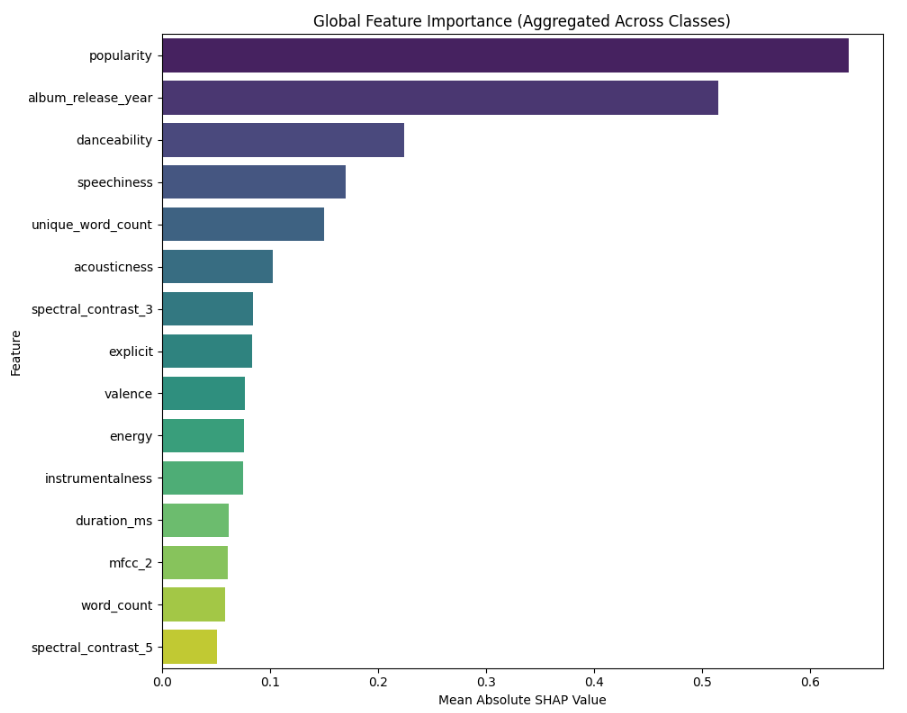
\includegraphics[width=6in]{img/feature_importance_genre_clf.png}
  \caption{SHAP feature importance plot of the classification model for genre
  trained on all features. The scores were averaged across all classes.}
  \label{Figure:feature_importance_genre_clf}
\end{figure}
\end{center}

SHAP global feature importance
plot (fig.~\ref{Figure:feature_importance_genre_clf}) for genre classification
shows that:
\begin{itemize}
  \item \textit{Popularity} and \textit{album release year} are the strongest
    predictors of \textit{genre}.  Possibly they capture trends and listener
    preferences linked to specific genres;
  \item Other key features included \textit{danceability},
    \textit{speechiness}, and \textit{unique word count}, which describe the
    style of the music and the content of the lyrics;
  \item Audio features like \textit{acousticness} and
    \textit{spectral contrast} also played a significant role, showing
    that the sound of the music indicates its genre;
  \item The \textit{explicit} flag also had a noticeable effect, which makes
    sense given its strong connection to genres like rap and hip-hop.

\end{itemize}

%---------------------------------------------------------------------------


\section{Topics Modeling}
\label{sec:topicsmodeling}

\subsection{Latent Dirichlet Allocation}

Latent Dirichlet Allocation (LDA) was applied to the song lyrics dataset to
identify thematic clusters and analyze the distribution of topics across songs.
The \textit{pyLDAvis} library that was used for this analysis generates topic
visualizations and facilitates uncovering the most prominent words in each
topic.\cite{pylda}

\begin{center}
\begin{figure}[H]
  \centering
  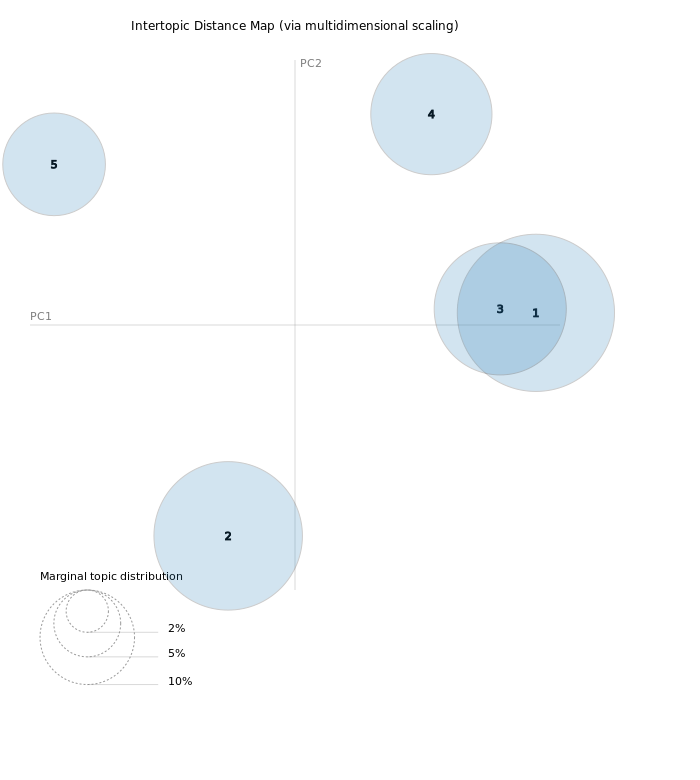
\includegraphics[width=6in]{img/topics/png/topics.png}
  \caption{Intertopic Distance Map.}
  \label{Figure:intertopicdistancemap}
\end{figure}
\end{center}

\begin{itemize}
  \item The bubble chart shows the intertopic distance map
    (fig.~\ref{Figure:intertopicdistancemap}) using multidimensional scaling
    (MDS). Each bubble represents a topic extracted by the LDA model;
  \item The position of the bubbles represents the relationship between topics.
    Topics closer together share more words or themes;
  \item The size of the bubbles represents the popularity of the topic within
    the entire dataset. The larger the bubble the higher the proportion of
    terms in the dataset.
\end{itemize}



\begin{center}
\begin{figure}[H]
  \centering
  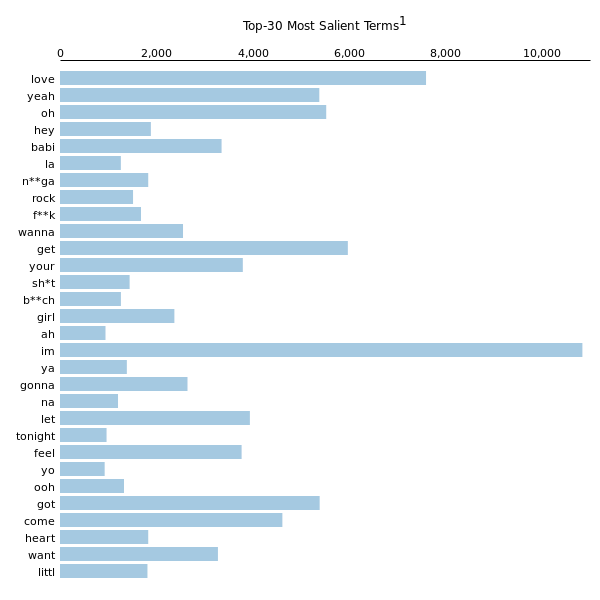
\includegraphics[width=6in]{img/topics/png/general.png}
  \caption{Top-30 Most Salient Terms across the entire corpus. The bars
  represent how often each term appears in the entire corpus.}
  \label{Figure:lda_general}
\end{figure}
\end{center}

\textbf{Blue bars on figure fig.~\ref{Figure:lda_general} show overall
frequency of the terms in the entire corpus. Red bars indicate estimated
frequency of the terms in that topic.} The results for each topic are presented
on figures fig.~\ref{Figure:t1}, fig.~\ref{Figure:t2}, fig.~\ref{Figure:t2},
fig.~\ref{Figure:t3}, fig.~\ref{Figure:t4}, fig.~\ref{Figure:t5},:

\begin{center}
\begin{figure}[H]
  \centering
  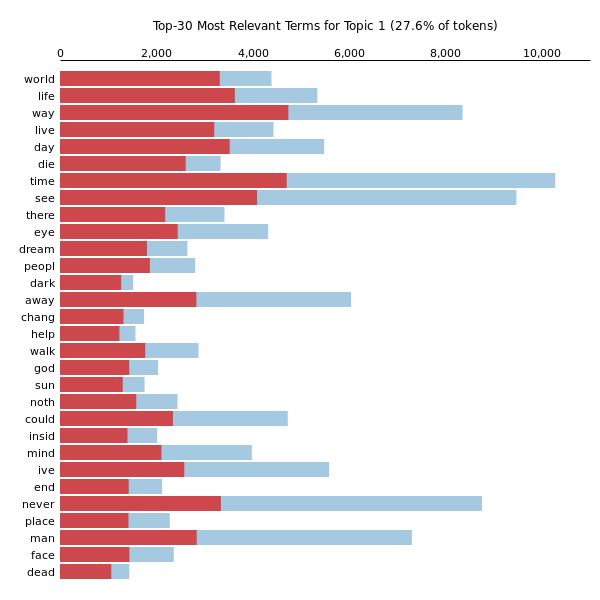
\includegraphics[width=6in]{img/topics/png/t1.png}
  \caption{Top-30 Most Relevant Terms in Topic 1.}
  \label{Figure:t1}
\end{figure}
\end{center}

\begin{center}
\begin{figure}[H]
  \centering
  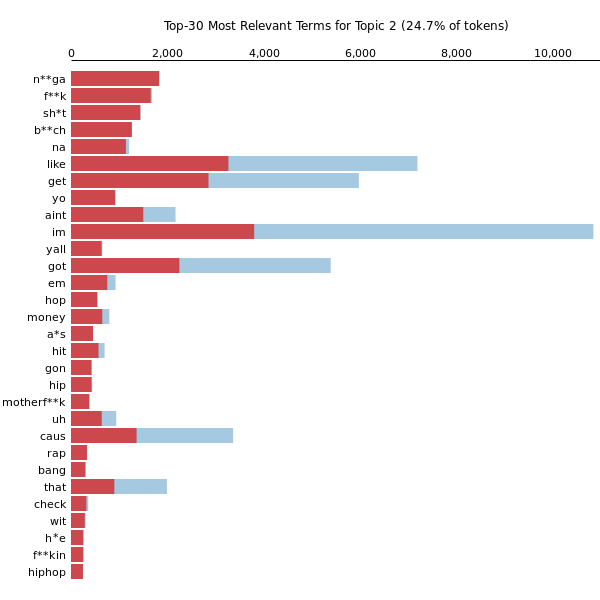
\includegraphics[width=6in]{img/topics/png/t2_censored.png}
  \caption{Top-30 Most Relevant Terms in Topic 2.}
  \label{Figure:t2}
\end{figure}
\end{center}

\begin{center}
\begin{figure}[H]
  \centering
  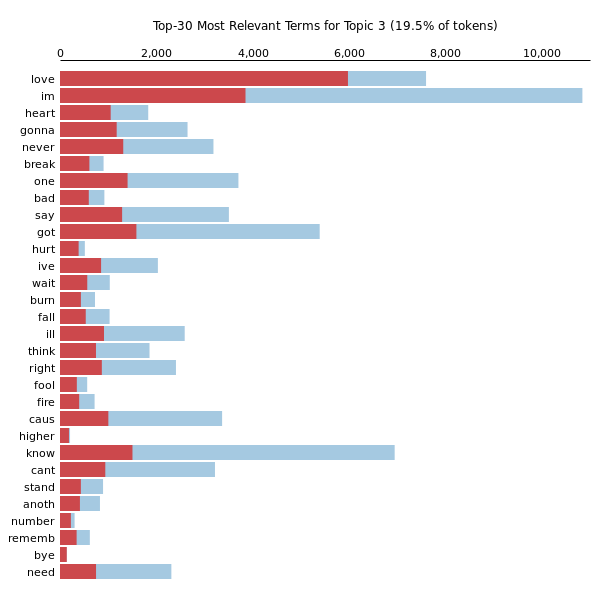
\includegraphics[width=6in]{img/topics/png/t3.png}
  \caption{Top-30 Most Relevant Terms in Topic 3.}
  \label{Figure:t3}
\end{figure}
\end{center}

\begin{center}
\begin{figure}[H]
  \centering
  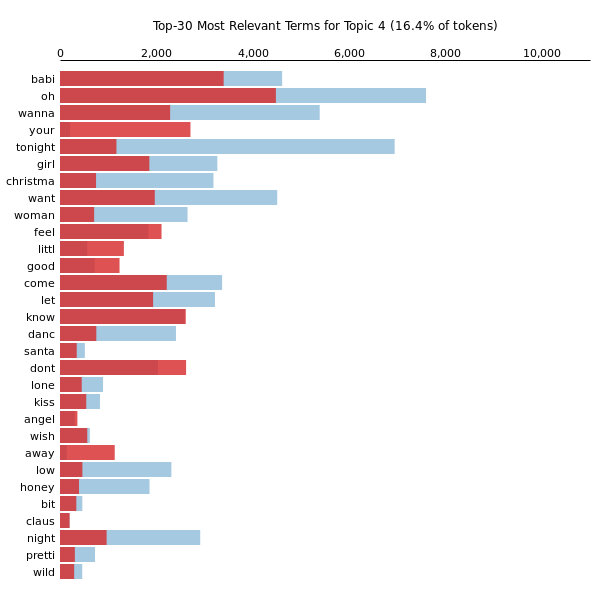
\includegraphics[width=6in]{img/topics/png/t4.png}
  \caption{Top-30 Most Relevant Terms in Topic 4.}
  \label{Figure:t4}
\end{figure}
\end{center}

\begin{center}
\begin{figure}[H]
  \centering
  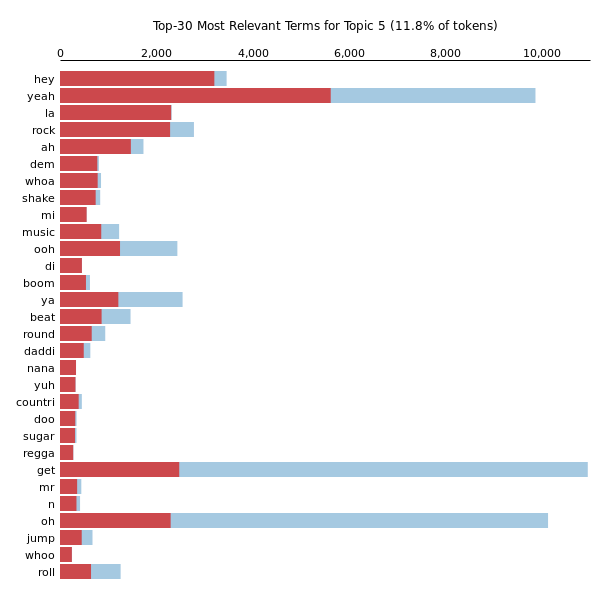
\includegraphics[width=6in]{img/topics/png/t5.png}
  \caption{Top-30 Most Relevant Terms in Topic 5.}
  \label{Figure:t5}
\end{figure}
\end{center}

LDA revealed distinct themes found in the corpus of  lyrics in the dataset. It
identified five well separated themes, with overlaps only in highly related
topics, such as existentialism (Topic 1) and emotional conflict (Topic 3).
Their similarity is visualized on the intertopic
(fig~\ref{Figure:intertopicdistancemap}) distance map. Topics with overlap have
many terms in common. Based on the visualizations (fig.~\ref{Figure:t1},
fig.~\ref{Figure:t2}, fig.~\ref{Figure:t3}, fig.~\ref{Figure:t4},
fig.~\ref{Figure:t5}) we can observe that:

\begin{itemize}
     \item Topic 1 represents \textbf{philosophical and existential} themes in lyrics.
      Top words in that topic include ``world'', ``life'', ``time'', ``die'',
      ``live'', and ``dream'';
    \item Topic 2 is characterized by \textbf{colloquial and explicit
      language}. It likely represents themes related to \textbf{rap and hip hop culture}
      and seems to be strongly tied to urban and street culture themes;
    \item Topic 3 revolves around themes of \textbf{love, heartbreak, emotional
      conflict and relationships}, as indicated by words like ``love'',
      ``heart'', ``hurt'', ``break'';
    \item Topic 4 focuses on themes of \textbf{romantic affection, celebration,
      and festives}. Words such as ``baby'', ``tonight'', ``girl'', ``wanna'',
      and ``kiss'' indicate intimate emotions and the presence of
      ``Christmas'', ``Santa'' and other related words strongly suggests a
      Christmas-themed music;
    \item Topic 5 appears to center around themes of \textbf{music, rhythm and
      energetic expressions}. Most prominent words identified for that topic
      are ``hey'', ``yeah'', ``rock'', ``music'' and ``beat''. They suggest a
      focus on the sound and feel of music. 
\end{itemize}


\subsection{Genre Distribution Across Topics}
These results demonstrate the potential of topic modeling to extract and
analyze dominant lyrical themes in music at scale. After assigning the most
probable topic to each song the distribution of features and genres in each
topic can be checked.


\begin{center}
\begin{figure}[H]
  \centering
  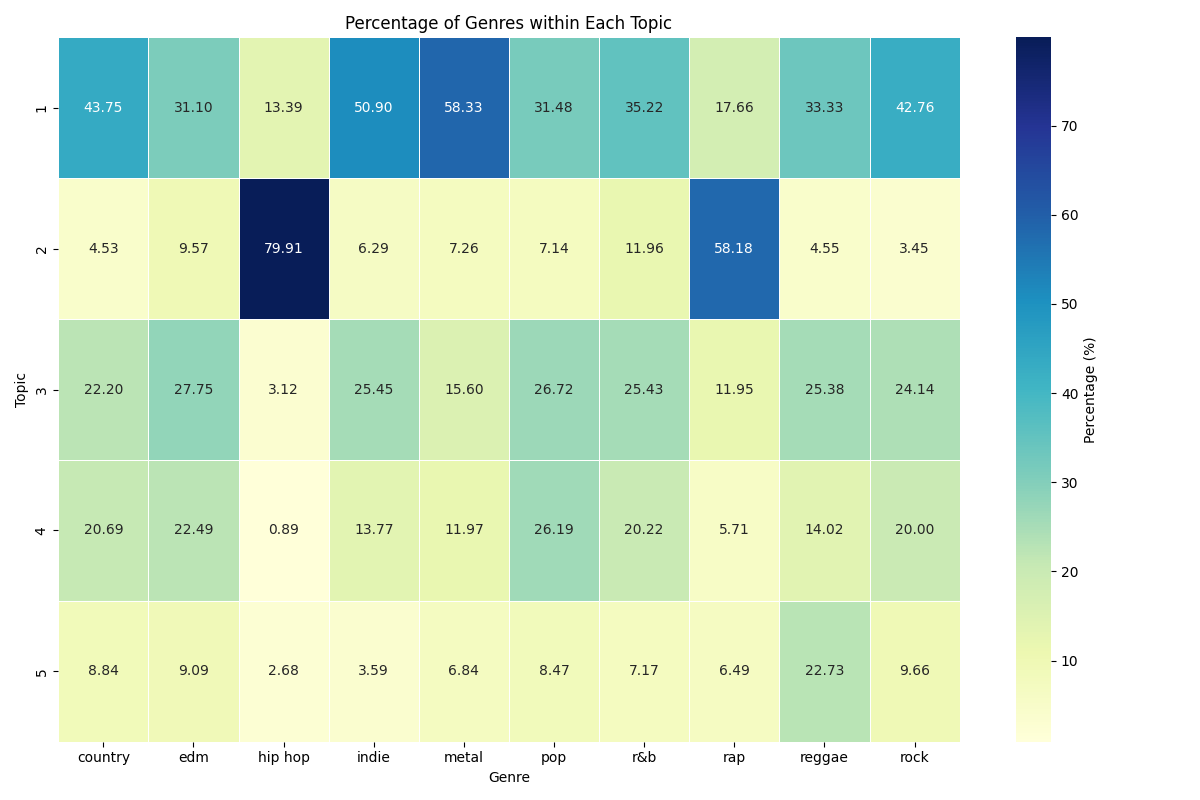
\includegraphics[width=6in]{img/lda_genres_distribution.png}
  \caption{Heatmap showing percentage of genres in each topic.}
  \label{Figure:lda_genres_distribution}
\end{figure}
\end{center}

The heatmap (fig.~\ref{Figure:lda_genres_distribution}) shows the percentage
distribution of genres within each topic extracted with the LDA model. Key
observations include:

\begin{itemize}
  \item \textbf{Topic 1} has a balanced distribution across multiple genres,
    with slight overhead of \textit{metal};
  \item \textbf{Topic 2} is dominated by \textit{rap} and \textit{hip hop}
    genres, which aligns with its themes of urban culture and colloquial
    language;
  \item \textbf{Topic 3} focuses on love and heartbreak, a common theme in
    music across many genres. The heatmap doesn't show any dominant genre, with
    \textit{R\&B}, \textit{rock}, \textit{pop}, and \textit{country} making the
    highest contributions;
  \item \textbf{Topic 4} has a significant representation in \textit{R\&B},
    \textit{pop} and \textit{country}, which suggests its romantic and festive
    focus;
  \item \textbf{Topic 5} seems to be linked to \textit{reggae} and
    \textit{rock}.
\end{itemize}

Based on the heatmap, topics 1 and 3 show more diverse genre distribution,
indicating thematic universality or overlap. This observation aligns with the
conclusions drawn from the  distance map
(fig.~\ref{Figure:intertopicdistancemap}) and the analysis of their most
relevant terms (fig.~\ref{Figure:t1}, fig.~\ref{Figure:t3}). Topics 2
(fig.~\ref{Figure:t2}) and 5 (fig.~\ref{Figure:t5}) display strong dominance by
specific genres, showing more focused thematic expressions.


\subsection{Empath Features Distributions Across Topics}

\begin{center}
\begin{figure}[H]
  \centering
  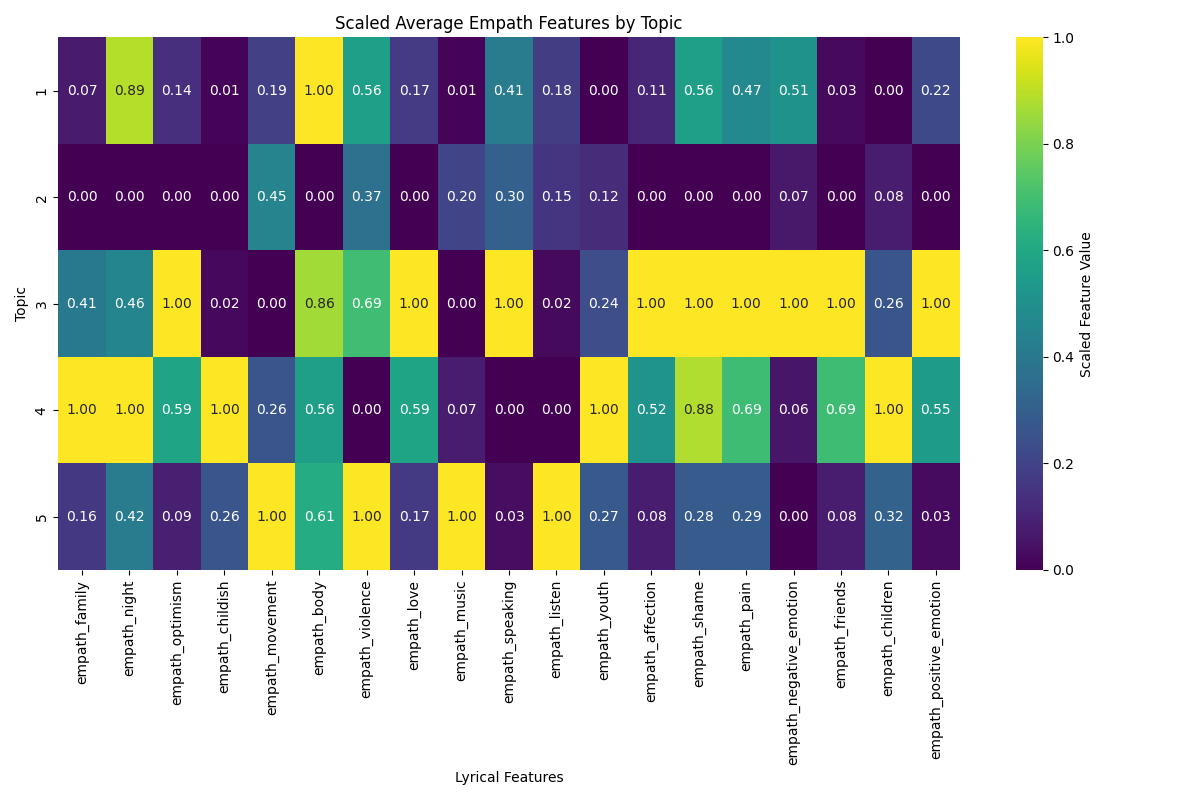
\includegraphics[width=6in]{img/lda_empath_features.png}
  \caption{Heatmap showing the distribution of scaled empath features across topics.}
  \label{Figure:lda_empath_features}
\end{figure}
\end{center}


This heatmap (fig.~\ref{Figure:lda_empath_features}) shows the scaled average
empath features by topic. It visualizes the significanace of specific lyrical
themes within each topic. 

\noindent \noindent Key observations:

\begin{itemize}
  \item \textbf{Topic 1}: high values of \textit{night}, \textit{body},
    \textit{pain} and \textit{shame} suggest lyrics focusing on darker or more
    aggresive themes, which aligns well with the dominance of metal as the main
    genre;
  \item \textbf{Topic 2}: strong connection with \textit{violence},
    \textit{movement}, \textit{speaking} and \textit{youth}, which are themes
    frequently occurring themes in rap and hip hop music;
  \item \textbf{Topic 3}: Strong emphasis on \textit{love}, \textit{affection},
    \textit{negative emotions}, and \textit{friends} indicates themes of
    relationships, heartbreak, and emotional conflict;
  \item \textbf{Topic 4}: High values for \textit{family}, \textit{children},
    \textit{positive emotions}, and \textit{youth} suggest themes of affection
    and relationships with loved ones, aligning well with previously identified
    possible relation to festives like Christmas;
  \item \textbf{Topic 5}: High values in \textit{music}, \textit{movement}, and
    \textit{violence} suggest rhythmic and energetic themes.
\end{itemize}

\subsection{Sentiment Across Topics}
\begin{center}
\begin{figure}[H]
  \centering
  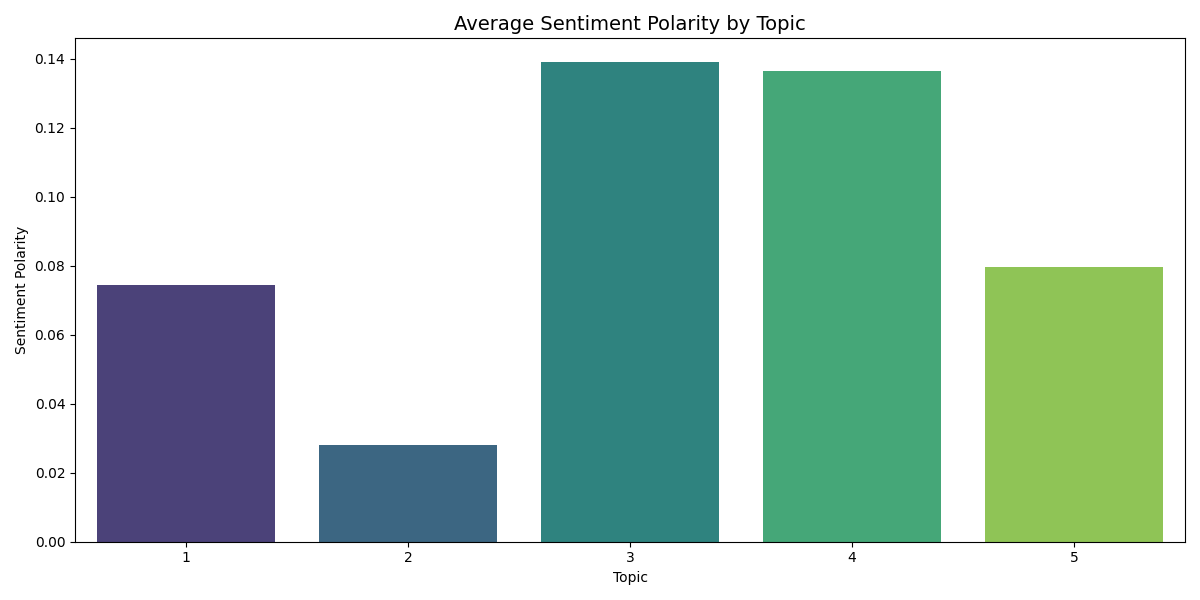
\includegraphics[width=6in]{img/lda_sentiment.png}
  \caption{Bar chart showing average sentiment polarity by topic.}
  \label{Figure:lda_sentiment}
\end{figure}
\end{center}

The average sentiment polarity bar chart (fig.~\ref{Figure:lda_sentiment}) illustrates the positiveness for each
topic. Topics 3 and 4 have the highest sentiment polarity, which indicates more
positive themes. Topic 2 has the lowest average, indicating more negative
lyrics sentiment, which aligns with previous findings.

\subsection{Spotify Features Across Topics}

\begin{center}
\begin{figure}[H]
  \centering
  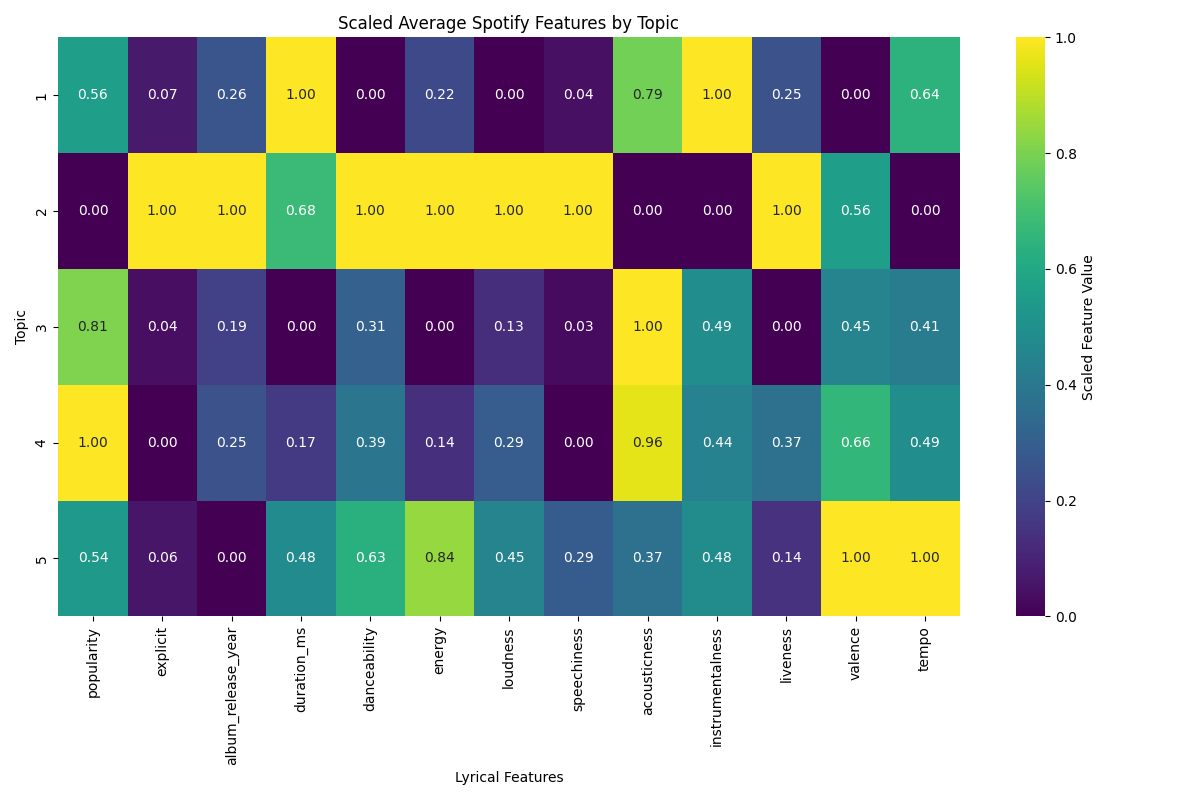
\includegraphics[width=6in]{img/lda_spotify_features.png}
  \caption{Heatmap showing average values of scaled spotify features in each
  topic.}
  \label{Figure:lda_spotify_features}
\end{figure}
\end{center}

The heatmap (fig.~\ref{Figure:lda_spotify_features}) shows a visualization of
the average scaled Spotify features across topics. It shows patterns for each
topic and describes their unique musical attributes:

\begin{itemize}
  \item \textbf{Topic 1}: High values in \textit{acousticness},
    \textit{instrumentalness} and low \textit{danceability} and
    \textit{valance} suggest calmer, more instrumental tracks;
  \item \textbf{Topic 2}: High values in \textit{explicitness},
    \textit{speechiness}, \textit{liveness}, \textit{energy} and
    \textit{loudness} suggest tracks with strong vocal content, high energy
    and explicit language, aligning well with the dominant genres in this
    topic;
  \item \textbf{Topic 3}: High \textit{popularity} and \textit{acousticness},
    with low \textit{energy} and  \textit{danceability} suggest slower,
    more emotional, acoustic tracks;
  \item \textbf{Topic 4}: High \textit{acousticness},  \textit{popularity},
    relatively high \textit{valence} and \textit{tempo} indicate softer and
    very acoustic songs;
  \item \textbf{Topic 5}: High values in \textit{tempo}, \textit{valence}, and
    \textit{danceability}, along with moderate \textit{energy}, suggest
    energetic and possibly danceable tracks.
\end{itemize}

\clearpage
\section{Temporal Trends in Music}
\label{sec:temporaltrends}

To analyze the temporal trends in musical features, during the data collection
phase the variable \textit{album release year} was stratified into 10-year
buckets representing distinct decades. This stratification allowed for a
comparative analysis of feature evolution across time periods, assuring
that each time period had sufficient representation.


\subsection{Identification of Features Affected by Release Year}

In order to identify the features that changed significantly over the decades
two tests were conducted:


\begin{itemize}
  \item \textbf{Linear Regression Analysis}: Simple linear regression models
    were trained for each feature using the decade as the independent variable.
    The values of coefficient of determination ($R^2$) indicated how well the
    decade explained the variance in each feature;
  \item \textbf{ANOVA Testing}: Analysis of variance (ANOVA) was conducted for
    each feature to verify if the feature mean in at least one of the decades
    was different.
\end{itemize}

Based on the table Tab.~\ref{Table:trend_table}, features with high $R^2$
values and statistically significant p-values ($\alpha = 0.05$) from ANOVA were
selected as candidates for further analysis. In total 24 features were
identified as having meaningful relationship with the decade of release. Their
$R^2$ and p-values can be seen in the table Tab.~\ref{Table:trend_table}:


% \usepackage{color}
% \usepackage{tabularray}
\begin{table}[H]
\centering
\caption{Features identified as having significant dependency on the decade of
release.}
\label{Table:trend_table}
\begin{tblr}{
  column{even} = {r},
  column{3} = {r},
  column{5} = {r},
  hline{1,25} = {-}{0.08em},
  hline{2} = {-}{},
}
\textbf{Feature}       & \textbf{R²} & \textbf{Trend Coefficient} & \textbf{F-Statistic} & \textbf{p-Value} \\
explicit               & 0.909073    & 0.006645                   & 76.023316            & 0.000000         \\
valence                & 0.906611    & -0.003028                  & 45.487845            & 0.000000         \\
syntactic\_complexity  & 0.905622    & 0.519760                   & 3.188473             & 0.002285         \\
popularity             & 0.893476    & 0.276672                   & 61.320459            & 0.000000         \\
vader\_compound        & 0.880113    & -0.007787                  & 11.830054            & 0.000000         \\
sentiment\_polarity    & 0.853502    & -0.001479                  & 8.135521             & 0.000000         \\
loudness               & 0.833296    & 0.068308                   & 139.657491           & 0.000000         \\
rhyme\_density         & 0.824603    & -0.000094                  & 18.454532            & 0.000000         \\
danceability           & 0.814174    & 0.001072                   & 7.099057             & 0.000000         \\
speechiness            & 0.806721    & 0.000817                   & 18.774707            & 0.000000         \\
dale\_chall            & 0.775952    & 0.031306                   & 5.824913             & 0.000001         \\
flesch\_reading\_ease  & 0.771849    & -0.415172                  & 3.364072             & 0.001401         \\
gunning\_fog           & 0.758302    & 0.154463                   & 3.178465             & 0.002350         \\
lexical\_richness      & 0.565358    & -0.000709                  & 10.507191            & 0.000000         \\
type\_token\_ratio     & 0.565358    & -0.000709                  & 10.507191            & 0.000000         \\
energy                 & 0.518081    & 0.003036                   & 84.094129            & 0.000000         \\
acousticness           & 0.469885    & -0.005867                  & 221.629618           & 0.000000         \\
duration\_ms           & 0.151967    & 495.225838                 & 102.202431           & 0.000000         \\
semantic\_depth        & 0.115761    & 0.000821                   & 3.334177             & 0.001523         \\
tempo                  & 0.110478    & 0.036494                   & 2.943202             & 0.004482         \\
sentiment\_variability & 0.064628    & -0.000182                  & 5.719228             & 0.000001         \\
linguistic\_uniqueness & 0.020538    & 0.000049                   & 2.558628             & 0.012530         \\
instrumentalness       & 0.016573    & 0.000118                   & 4.748720             & 0.000025         
\end{tblr}
\end{table}


\subsection{Plots and Results}
Figures fig.~\ref{Figure:trends1}, fig.~\ref{Figure:trends2} and
fig.~\ref{Figure:trends3} show the trends of these features across
decades,with 95\% confidence intervals to illustrate the variability of the
trends:

\begin{center}
\begin{figure}[H]
  \centering
  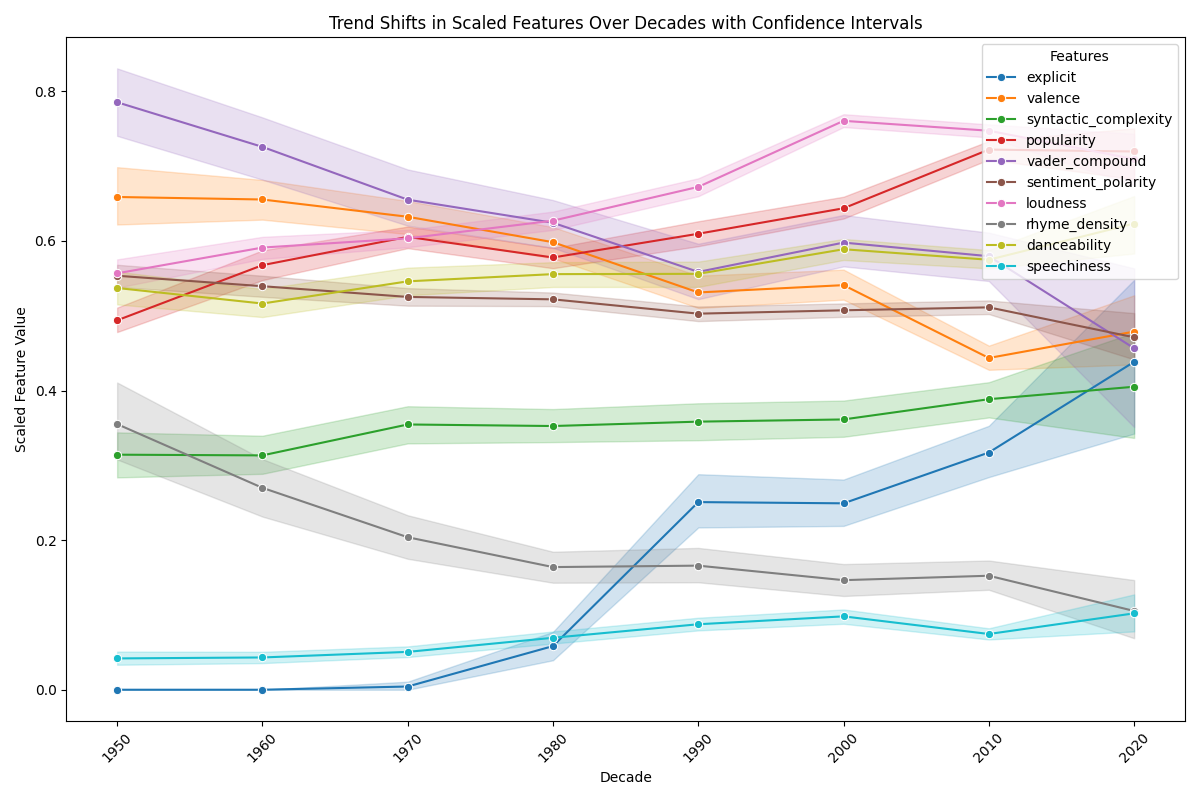
\includegraphics[width=6in]{img/temporal_trends_1.png}
  \caption{Plot showing temporal changes of features dependent on the decade in
  which the song was released.}
  \label{Figure:trends1}
\end{figure}
\end{center}

\begin{center}
\begin{figure}[H]
  \centering
  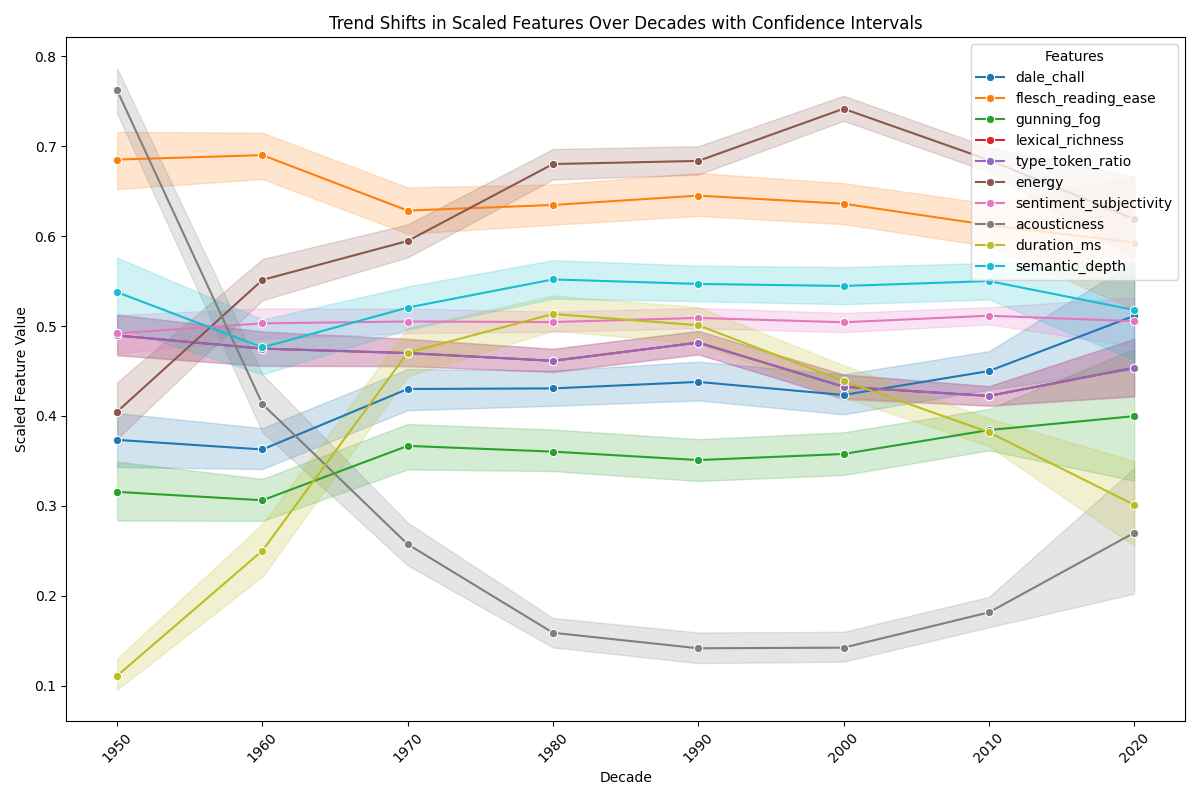
\includegraphics[width=6in]{img/temporal_trends_2.png}
  \caption{Plot showing temporal changes of features dependent on the decade in
  which the song was released.}
  \label{Figure:trends2}
\end{figure}
\end{center}

\begin{center}
\begin{figure}[H]
  \centering
  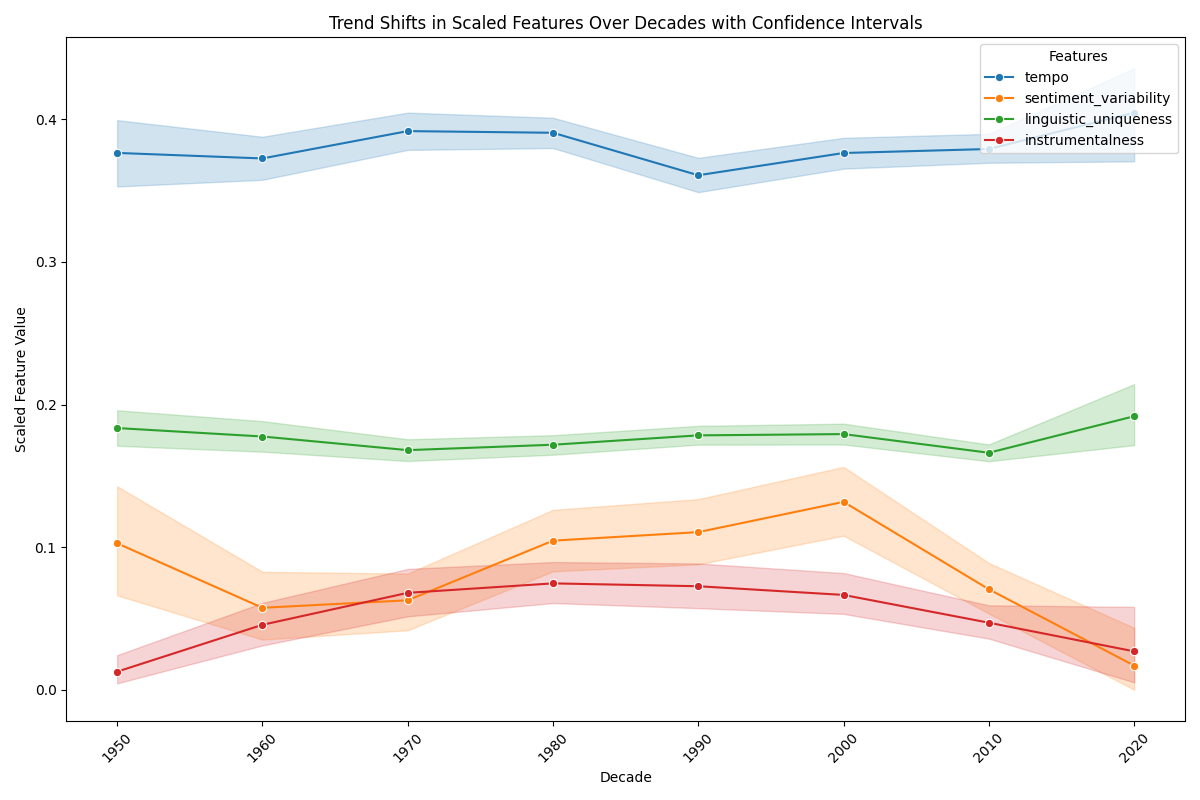
\includegraphics[width=6in]{img/temporal_trends_3.png}
  \caption{Plot showing temporal changes of features dependent on the decade in
  which the song was released.}
  \label{Figure:trends3}
\end{figure}
\end{center}

Based on those plots it can be observed that:
\begin{itemize}
  \item \textbf{There is a clear, strong upward trend in explicit content from
    the 1980s onward}. It reflects a cultural shift  towards more openness in
    lyrical expression and increase in popularity of genres such as rap;
  \item \textbf{ There is a steady increase in popularity over the decades.
    Potentially it might reflect increased focus on  producing music for mass
  appeal}, much like most of content created in the internet era;
  \item Speechiness peaks in the 1990s and 2000s, likely reflecting the rise of
    rap and spoken-word music during this period;
  \item Music seems to have shifted to less  positive songs over the decades, as
    indicated by the decrease in vader compound and valence;
  \item \textbf{There is a significant decrease in acousticness and
      an increase in energy over the decades, showing a clear
      shift in musical trends. This change could possibly correspond to
      the move away from acoustic to electronically produced music, with the
      rise of genres like EDM and modern pop};
  \item Loudness increased consistently over the decades, likely also
    influenced by the shift toward electronic music, which often includes
    amplified and dynamically intense production techniques.
\end{itemize}
